\chapter{Generating Adversarial Data}
\section{Background}
\subsection{Definitions}
\begin{figure}[h]
	\centering
	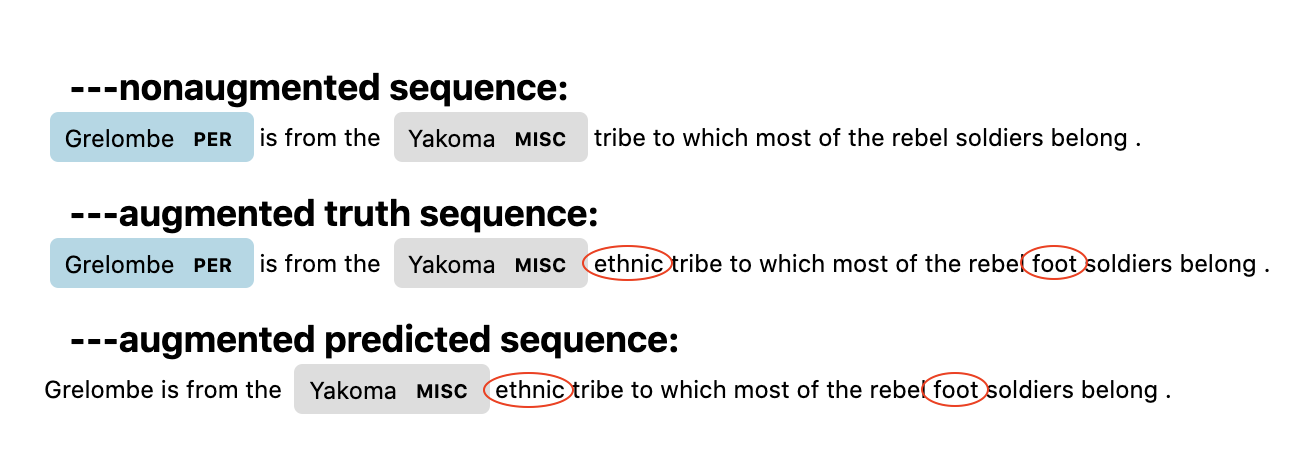
\includegraphics[width=0.95\linewidth]{LatexDiss/figures/insertmotivatingexample.png}
	\caption{Motivating example of a context-based adversarial attack. The first sentence is from the original CoNLL03 dataset. The second sentence is the correct labeling sequence. The third sentence is what the model predicted.}
	\label{fig:motivatingexampleinsert}
\end{figure}


As described in Sec~\ref{sec:introadv}, an adversarial example for a neural network is an example that is created by perturbing a correctly classified example, causing the model to misclassify the adversarial example. I explore several ways to perturb sentences such that the original entity labels and the sentence structure remain valid. These adversarial attacks include entity-based attacks -- masking entities and switching entities -- and context-based attacks -- inserting and removing adjectives as well as replacing non-entity words with synonyms. 

A motivating example of a context-based attack is seen in Fig~\ref{fig:motivatingexampleinsert}. In this adversarial attack, two adjectives are inserted into the sentence. Although the adversarial sentence has the exact same meaning as the original sentence, the model misses a \textsc{PER} entity label in the adversarial sentence despite correctly labeling the original sentence.

Fig~\ref{fig:motivatingexampleswitch} is a motivating example for an entity-based attack. In this attack, two \textsc{LOC} entities were switched between sentences. Despite predicting correctly on the two original sentences, the model predicted incorrectly on the adversarial sentence, classifying ``VANCOUVER'' as an \textsc{ORG} instead of a \textsc{LOC}.

\begin{figure}[h]
	\centering
	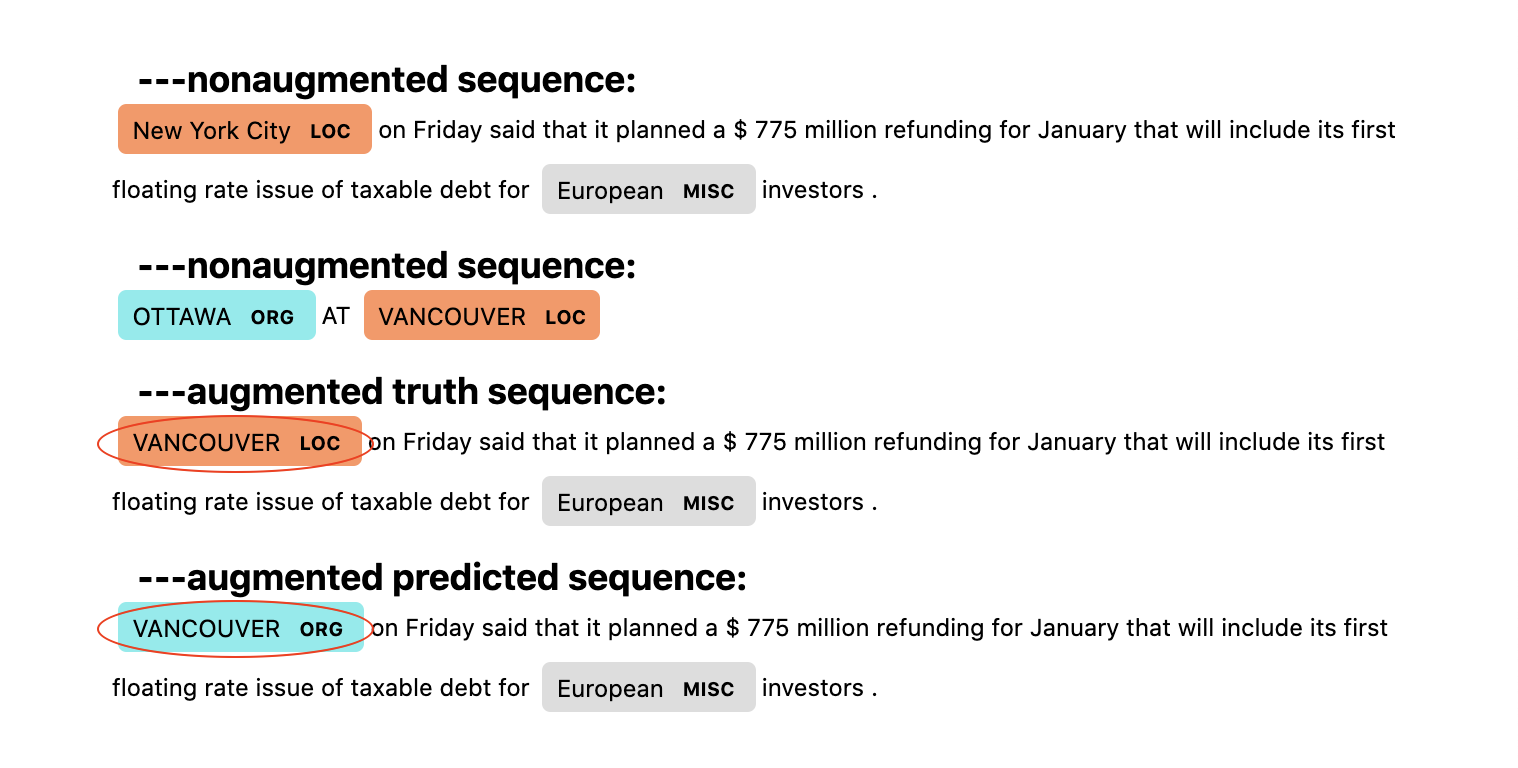
\includegraphics[width=1\linewidth]{LatexDiss/figures/LOCmotivatingexample.png}
	\caption{Motivating example of an entity-based adversarial attack. The first two sentences are from the original CoNLL03 dataset. The third sentence is the correct labeling sequence. The fourth sentence is what the model predicted.}
	\label{fig:motivatingexampleswitch}
\end{figure}


As described in Sec~\ref{sec:ourframework}, I use a BLSTM-CRF neural NER model throughout these experiments. I use CoNLL03 as the dataset for my experiments due to its pervasiveness throughout NER literature and its simplistic structure, having only four entity categories.

\subsection{Motivation}
An important question when evaluating a NER model is how well it will work in a real-world scenario. Because training, test, and dev data are usually collected in the same manner, the test data may be over-familiar to the NER model, causing the model to perform better on the test data than it might have on a completely different corpus during a real-world application. 

One cause of this discrepancy is that models rely heavily on memorizing named entities, meaning that they have difficulty generalizing to unseen entities. This memorization is evidenced in Table~\ref{tab:seenvsunseen} and Fig~\ref{fig:seenvsunseen}, which show that our baseline model performs significantly better given sentences with previously seen entities rather than sentences with only new entities. To test this, I split the CoNLL03 test data into two subsets, one having all of the sentences containing one or more entity from the training data, and the other having all of the sentences with only unseen entities.

 \begin{table}[h]
    \centering
    \begin{singlespace}
    \scalebox{.7} {
    \begin{tabular}{@{} R{0.3\textwidth}@{\hskip .6in} c c c | c c c @{}}
\toprule   \toprule
        & \multicolumn{3}{C{0.3\textwidth}}{\small{\textbf{Performance on dev data}}}
        & \multicolumn{3}{C{0.3\textwidth}}{\small{\textbf{Performance on test data}}} \\

        \small{\textbf{Subset of unlabeled data}}
        & \small{\textit{Precision}}
        & \small{\textit{Recall}}
        & \small{\textit{F1}}
        & \small{\textit{Precision}}
        & \small{\textit{Recall}}
        & \small{\textit{F1}} \\
\toprule
        \small{All sentences}
            & 94.86 & 94.5 & 94.68
            & 91.03 & 90.91 & 90.97 \\
        \small{One or more seen ents}
            & 96.93 & 96.84 & 96.88 &
            94.24 & 94.13 & 94.18 \\
        \small{Only unseen ents}
            & 90.17 & 88.82 & 89.49 & 
            87.66 & 85.86 & 86.75 \\
            
\hline
    \end{tabular}
    }
    \end{singlespace}
    \caption{Comparison of the our baseline model's performance on the standard CoNLL03 test data, the subset of the test data with at least one entity from the training data, and the subset of the test data with only unseen entities.}
    \label{tab:seenvsunseen}
\end{table}


\begin{figure}[h]
	\centering
	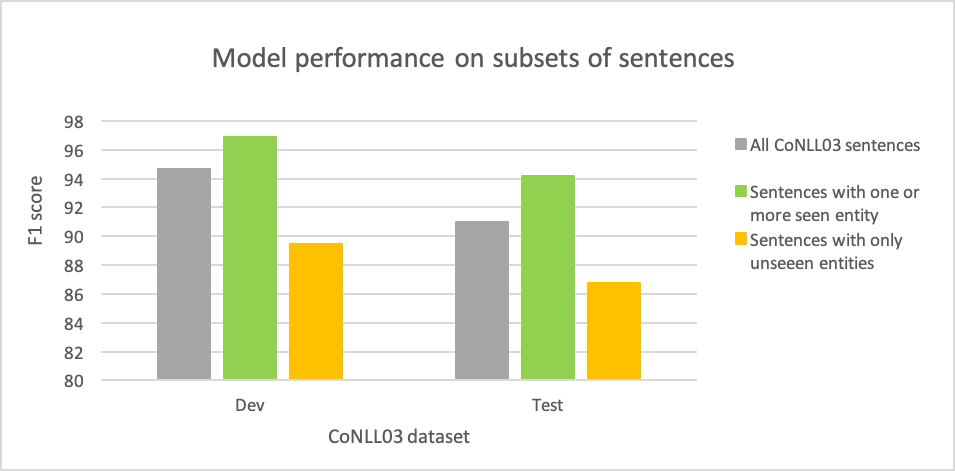
\includegraphics[width=0.85\linewidth]{LatexDiss/figures/seenvsunseen.png}
	\caption{Comparison of the our baseline model's performance on the standard CoNLL03 test data, the subset of the test data with at least one entity from the training data, and the subset of the test data with only unseen entities.}
	\label{fig:seenvsunseen}
\end{figure}

In order to further test a model's dependence on known entities, I develop adversarial sentences in which the entities are masked with random letters, and I develop adversarial sentences in which the entities are swapped between sentences.

Another reason that a NER model might perform worse on a new dataset is that the writing style is different  from the training set. Because NER models are generally trained and tested on data from the same corpus, their results can be overconfident in their ability to label new sentences. In order to test whether the model is overfitted to the writing style of the dataset, I develop adversarial sentences in which non-entities are manipulated. In particular, I remove adjectives, insert adjectives, and replace words with synonyms.

The main motivation for this work is developing schemes to create adversarial test data so that state-of-the-art models can be more accurately evaluated. An accurate evaluation will allow researchers to better understand in what circumstances it is safe to deploy state-of-the-art NER models. Additionally, these adversarial examples can shed light on the models' shortcomings, pointing future research in a productive direction. A secondary motivation for this work is using adversarial data to benefit the models. I investigate the effectiveness of adversarial training -- training the models on adversarial training examples -- to develop more robust models.


\section{Adversarial Attack Experiments}
\label{sec:advattackexp}
In this section, I describe the different types of adversarial attacks I experiment with and examine their effectiveness. For each attack type, I develop a script to augment an input dataset in an adversarial manner. For example, the entity masking script takes a standard dataset as input and returns the same dataset with each entity replaced by a random string of characters. I run these augmentation scripts on the CoNLL03 datasets to produce augmented dev and test datasets. I then train a NER model on the original CoNLL03 training and dev set and test its ability to correctly label the augmented dev and test datasets. The results on the augmented test datasets are particularly meaningful because the test set is not used anywhere in the training of the model, so its sentences are completely new to the NER model. I find that our baseline NER model performs worse on these adversarial datasets than on the original CoNLL03 dev and test set, evidencing the success of my adversarial attacks in demonstrating a lack of robustness in state-of-the-art NER models.

\subsection{Entity-based attacks}
\subsubsection{Full Entity Masking}
The most straightforward approach I took was fully masking every entity in a given sentence. To form a mask, I replaced each letter in the entity with a random letter with the same case (to retain the same capitalization). Any non-alphabetic characters (e.g. hyphens or digits) were left the same. 

Masking entities drastically affected the model's performance, causing the model to achieve an F1 score of 61.66\% compared to 90.97\% on the original test data. In fact, this attack may perform too well, changing the sentence to an extent that would make labeling it too difficult even for humans. For example, one of the sentences in the entity-swapped data reads \textit{``Kelyta feedlot cattle roundup -- RZIJ.''}. This corresponds to the original sentence \textit{``Kansas feedlot cattle roundup -- USDA.''} In this example, even as a human we need the entity \textit{USDA} itself to understand the final word as an organization.

\subsubsection{Single-Entity Masking}
In order to address the problem of over-masking, I propose several strategies. First, I only mask one entity in a sentence. Often, when trying to label a given entity in a sentence, other nearby entities help to provide context. The single-entity masking approach allows for the context of other entities. As shown in Table~\ref{tab:entityattacksresults} and Fig~\ref{fig:entityattacksresults}, masking a single entity per sentence still successfully reduces the model's performance, while reducing it to a more realistic extent, from a 90.97\% F1 score to 84.63\%.

Within the two categories of single-entity masking and full entity masking, I test three different masking approaches. The first method is fully masking every letter as described above.

\subsubsection{Half Masking}
 My second approach is half masking, in which I only mask every other letter in an entity. As with full masking, I retain casing and special characters. For example, the original sentence \textit{``SOCCER - JAPAN GETS LUCKY WIN, CHINA IN SUPRISE DEFEAT.''} is masked to \textit{``SOCCER - JPPZN GETS LUCKY WIN, CKIKA IN SUPRISE DEFEAT.''}. As a human, I find this half masked sentence is easier to label than its fully masked counterpart \textit{``SOCCER - LNQUY GETS LUCKY WIN, INNXM IN SUPRISE DEFEAT.''} As shown in Table~\ref{tab:entityattacksresults} and Fig~\ref{fig:entityattacksresults}, partial masking allows the model to perform better than full masking, although the difference is small.
 
 \subsubsection{Masking with Retained Vowels}
 My final approach to masking is to mask the entire word, but only replace vowels with vowels and consonants with consonants. I came up with this approach in the hopes that the vowel/consonant pattern would retain enough morphological structure to help the model decipher the proper labels. However, I was surprised to find that there was almost no difference between the model's performance on fully masked sentences and sentences masked with the vowels retained (shown in Table~\ref{tab:entityattacksresults} and Fig~\ref{fig:entityattacksresults}).
 
 \subsubsection{Entity Switching}
 Along with masking entities, I created adversarial sentences by switching entities between sentences. Specifically, for every pair of entities of the same type in the corpus, I created two new sentences with the entities switched. That is, given a sentence $m = (m_{ne}, i)$ with non-entities $m_{ne}$ and entity $i$ and a sentence $n = (n_{ne}, j)$ with non-entities $n_{ne}$ and entity $j$, I produce two new sentences $m' = (m_{ne}, j)$ and $n' = (n_{ne}, i)$. The goal of this attack is to test if the model is memorizing the context for specific entities rather than the context for entity types. For example, the \texttt{PER} entity ``Michael Phelps'' might often be associated with words about swimming. If we switch ``Michael Phelps'' and ``Vin Diesel,'' putting Michael Phelps in a sentence about acting, can the model still recognize Michael Phelps as a \texttt{PER} entity? As can be seen in Table~\ref{tab:entityattacksresults} and Fig~\ref{fig:entityattacksresults}, entity switching had no significant effect on model performance.
 
 \subsubsection{Results of entity-based adversarial attacks}
  The results in Table~\ref{tab:entityattacksresults} and Fig~\ref{fig:entityattacksresults} demonstrate the effectiveness of entity masking in attacking our NER model, suggesting that the model relies heavily on entity memorization. The fact that entity switching was not an effective strategy suggests that the NER model does not focus on the context of specific entities. In order to validate these attacks, we will need to perform a human study to ensure that the generated sentences can still be labeled by humans. In this regard, it is likely that the entity masking attacks using only one entity are more realistic.
  
  \newpage
 
 \begin{table}[h]
    \centering
    \begin{singlespace}
    \scalebox{.7} {
    \begin{tabular}{@{} R{0.4\textwidth}@{\hskip .6in} c c c | c c c @{}}
\toprule   \toprule
        & \multicolumn{3}{L{0.3\textwidth}}{\small{\textbf{Performance on dev data}}}
        & \multicolumn{3}{L{0.3\textwidth}}{\small{\textbf{Performance on test data}}} \\

        \small{\textbf{Adversarial Technique}}
        & \small{\textit{Precision}}
        & \small{\textit{Recall}}
        & \small{\textit{F1}}
        & \small{\textit{Precision}}
        & \small{\textit{Recall}}
        & \small{\textit{F1}} \\
\toprule
        \small{Original data}
            & 94.86 & 94.50 & 94.68
            & 91.03 & 90.91 & 90.97 \\
\midrule
        \small{Entity Switching}
            & 93.99 & 93.62 & 93.81 
            & 91.37 & 90.47 & 90.92 \\
\midrule
        \small{All ents fully masked}
            & 62.89 & 58.60 & 60.67 
            & 63.94 & 59.54 & 61.66 \\
        \small{All ents half masked}
            & 65.26 & 61.76 & 63.46 
            & 66.16 & 62.20 & 64.12 \\
        \small{All ents masked, retain vowels}
            & 62.82 & 59.32 & 61.02 
            & 64.68 & 60.82 & 62.69 \\
\midrule
        \small{One ent fully masked}
            & 87.46 & 85.65 & 86.55 
            & 85.68 & 83.60 & 84.63 \\
        \small{One ent half masked} 
            & 88.01 & 86.58 & 87.29
            & 86.12 & 84.23 & 85.16 \\
        \small{One ent masked, retain vowels}
            & 87.54 & 86.04 & 86.79
            & 85.62 & 83.77 & 84.68 \\
            
\hline
    \end{tabular}
    }
    \end{singlespace}
    \caption{Comparison of our baseline model's performance on the standard CoNLL03 datasets with its performance on entity-based adversarial attacks.}
    \label{tab:entityattacksresults}
\end{table}

\begin{figure}[h]
	\centering
	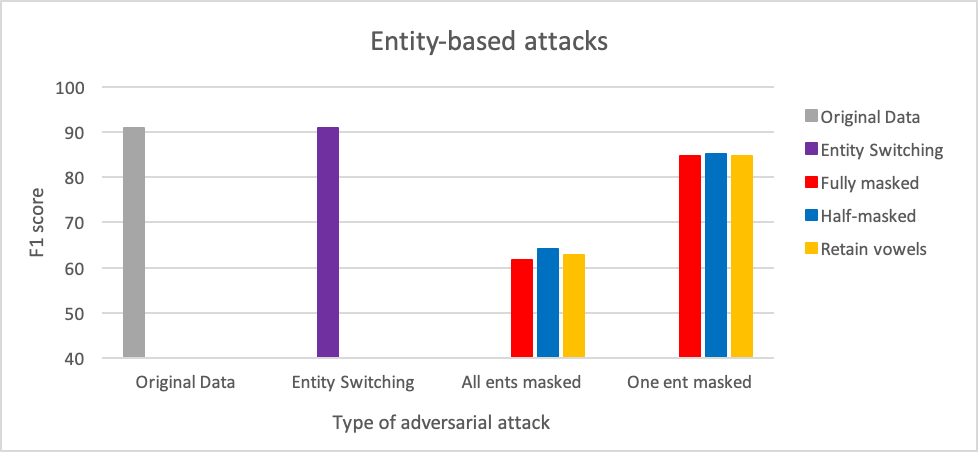
\includegraphics[width=0.85\linewidth]{LatexDiss/figures/entityattacks.png}
	\caption{Comparison of our baseline model's performance on the standard CoNLL03 test data with its performance on entity-based adversarial attacks.}
	\label{fig:entityattacksresults}
\end{figure}
 
 
\subsection{Context-based attacks}
In this section I focus on context-based attacks: adding non-entity adjectives before non-entity nouns, removing non-entity adjectives, and replacing non-entity words with synonyms. When choosing related words to insert or replace original words with, I mimic the existing casing pattern (all lowercase, all uppercase, or capitalized) in order to retain continuity with the rest of the sentence. Further, in order to decrease the chance of inserting a named entity, I don't allow suggested related words that were capitalized before this formatting.

Within these context-based attacks there are several subcategories based on two variables: how to choose which non-entity words to attack and how to select related words (necessary for inserting adjectives or replacing words with synonyms). Intuitively, I would like to attack the most influential words since the goal is to create a sentence that the model can no longer label properly. I investigate three different ways of choosing the most influential words: random selection, model differentiation, and cooccurrence matrices. I also use two different publicly-available platforms for selecting related words: ConceptNet and Bert.

\subsubsection{Selecting related words: ConceptNet}
The first technique for selecting related words that I explored is ConceptNet, a publicly-available semantic network, created to provide computers an understanding of the meaning of words \citep{conceptnet}. ConceptNet contains a massive dictionary of related words with a variety of relation types in many languages. For example, once ConceptNet is parsed to only show English words with relations relevant to my work, ``abandon synonym quit 1.0'' indicates that ``quit'' is a synonym for ``abandon'' with a confidence score of $1.0$. I also use the relation \textit{hasproperty} to find adjectives. For example, ``apple hasproperty red 9.592'' indicates that ``red'' is an adjective for apple. ConceptNet's \textit{hasproperty} relation also includes non-adjective phrases (such as ``antlers hasproperty shaped\_like\_trees,'' so I only use single-word properties.

A major downside to using ConceptNet for word manipulation is that it does not take the sentence context into account when selecting related words. As an example, the original CoNLL03 sentence \textit{``The presidential contest put the stock market in the twilight zone''} was changed to \textit{``The presidential contest put the broth market in the twilight zone''}. In this case, ``stock'' was changed to ``broth'' because they are synonyms in the context of soups. However, in the context of this sentence, the substitution does not make sense.

\subsubsection{Selecting related words: BERT}
\label{sec:BERT}
In order to use the full sentence as context when deciding on a replacement word, I used BERT's masked token prediction capability \citep{BERT}. BERT (Bidirectional Encoder Representations from Transformers) is an NLP model that can be fine-tuned for specific tasks, such as NER or question answering. In order to train a deep representation from unlabeled text, BERT is pre-trained by masking tokens in the unlabeled text and learning to predict those masked tokens \citep{BERT}. 

In order to get a related word, I mask the word I want a synonym of or insert a mask before the noun I want to add an adjective to. I then use BERT's masked token prediction functionality to generate a list of possible words for the mask. For example, if I wanted a synonym for ``stock'' in \textit{``The presidential contest put the stock market in the twilight zone.''} I would input the sentence \textit{``The presidential contest put the [MASK] market in the twilight zone.''}. In this example, BERT suggests the words ``entire'', ``local'', ``fish'', ``stock'', and ``black'', giving a corresponding confidence score for each. Of course, I cannot use ``stock'' because that was the original world. In contrast to ConceptNet, which suggested ``broth,'' BERT shows an understanding of the sentence's context.

Currently, I am using the suggested related word with the highest confidence rating, with the intuition that this is the most likely to form a valid sentence. However, my next direction will be to use lower-ranking words. My hypothesis is that these lower-ranking words will be more effective as adversarial attacks because they are less common words.

\subsubsection{Results of context-based attacks: related word selection}
As can be seen in Table~\ref{tab:relatedwords} and Fig~\ref{fig:relatedwords}, BERT's adversarial attacks tend to be more effective across a variety of experiments. The specifics of these experiments are explained in Sec~\ref{sec:randomselection} and Sec~\ref{sec:allennlpinterpret}. Additionally, BERT is more likely to create semantically meaningful sentences because it takes into account the context of a sentence, as discussed in Sec~\ref{sec:BERT}. For this reason, for the remainder of the experiments I only present results using BERT to select related words unless otherwise specified.

\begin{table}[h]
    \centering
    \begin{singlespace}
    \scalebox{.7} {
    \begin{tabular}{@{} R{0.6\textwidth}@{\hskip .6in} c c c | c c c @{}}
\toprule   \toprule
        & \multicolumn{3}{L{0.3\textwidth}}{\small{\textbf{Performance on dev data}}}
        & \multicolumn{3}{L{0.3\textwidth}}{\small{\textbf{Performance on test data}}} \\

        \small{\textbf{Adversarial Technique}}
        & \small{\textit{Precision}}
        & \small{\textit{Recall}}
        & \small{\textit{F1}}
        & \small{\textit{Precision}}
        & \small{\textit{Recall}}
        & \small{\textit{F1}} \\
\toprule
        \small{Original data}
            & 94.86 & 94.50 & 94.68
            & 91.03 & 90.91 & 90.97 \\
\midrule
        \small{Insert adjectives randomly (BERT)}
            & 88.46 & 82.63 & 85.45 
            & 86.03 & 85.4 & 85.71 \\
        \small{Insert adjectives randomly (ConceptNet)}
            & 93.10 & 85.71 & 89.26 
            & 87.10 & 90.00 & 88.52 \\
\midrule
        \small{Replace words randomly (BERT)} 
            & 93.35 & 92.79 & 93.07 
            & 90.30 & 89.33 & 89.81 \\
        \small{Replace words randomly (ConceptNet)} 
            & 95.44 & 94.96 & 95.20
            & 92.67 & 91.79 & 92.23 \\
\midrule
        \small{Insert adjectives using AllenNLP Interpret (BERT)}
            & 94.49 & 94.61 & 94.55
            & 90.88 & 90.79 & 90.83 \\
        \small{Insert adjectives using AllenNLP Interpret (ConceptNet)}
            & 93.71 & 94.29 & 94.00 
            & 90.99 & 90.76 & 90.87\\
\midrule
        \small{Replace words using AllenNLP Interpret (BERT)} 
            & 95.35 & 95.18 & 95.26
            & 92.89 & 92.12 & 92.50 \\
        \small{Replace words using AllenNLP Interpret (ConceptNet)} 
            & 95.91 & 95.80 & 95.86 
            & 93.28 & 92.99 & 93.13 \\
\hline
    \end{tabular}
    }
    \end{singlespace}
    \caption{Comparison of of BERT and ConceptNet for selecting related words. This experiment was performed using our baseline model and the CoNLL03 dataset.}
    \label{tab:relatedwords}
\end{table}
 
 \begin{figure}[h]
	\centering
	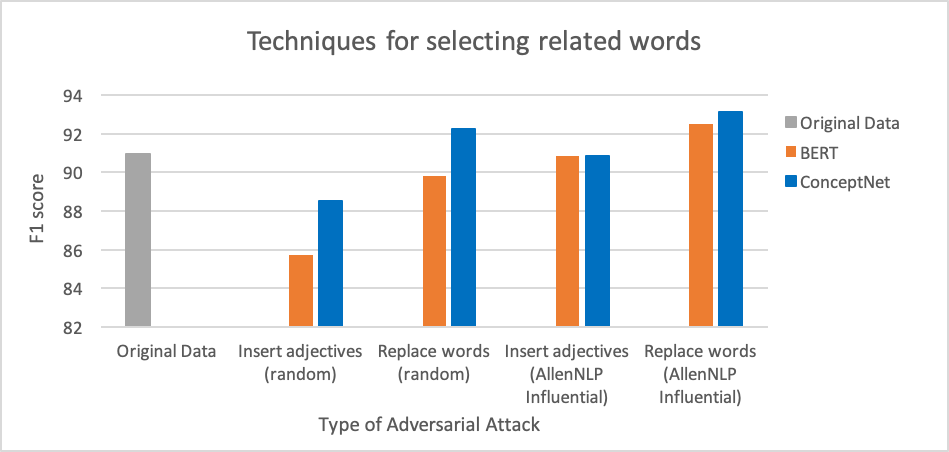
\includegraphics[width=0.85\linewidth]{LatexDiss/figures/relatedwords.png}
	\caption{Comparison of of BERT and ConceptNet for selecting related words. This experiment was performed using our baseline model and the CoNLL03 test set.}
	\label{fig:relatedwords}
\end{figure}


\subsubsection{Influential word selection: random}
\label{sec:randomselection}
The baseline for selecting influential words is to randomly select them. In order to investigate whether words closer to entities are more influential, I use two subcategories of random selection: manipulating words immediately preceding entities and manipulating words immediately preceding non-entities. As can be seen in Tab~\ref{tab:manipentsvsnonents} and Fig~\ref{fig:manipentsvsnonents}, the context-based adversarial attacks are more effective when words adjacent to entities are manipulated. For this reason, throughout this thesis random selection means randomly selecting words before entities unless otherwise specified.

\begin{table}[h]
    \centering
    \begin{singlespace}
    \scalebox{.7} {
    \begin{tabular}{@{} R{0.4\textwidth}@{\hskip .6in} c c c | c c c @{}}
\toprule   \toprule
        & \multicolumn{3}{L{0.3\textwidth}}{\small{\textbf{Performance on dev data}}}
        & \multicolumn{3}{L{0.3\textwidth}}{\small{\textbf{Performance on test data}}} \\

        \small{\textbf{Adversarial Technique}}
        & \small{\textit{Precision}}
        & \small{\textit{Recall}}
        & \small{\textit{F1}}
        & \small{\textit{Precision}}
        & \small{\textit{Recall}}
        & \small{\textit{F1}} \\
\toprule
        \small{Original data}
            & 94.86 & 94.50 & 94.68
            & 91.03 & 90.91 & 90.97 \\
\midrule
        \small{Remove adjectives before ents}
            & 89.47 & 82.93 & 86.08 
            & 80.65 & 78.12 & 79.37 \\
        \small{Remove adjectives before non-ents}
            & 93.54 & 93.16 & 93.35 
            & 89.48 & 88.89 & 89.18 \\
\midrule
        \small{Insert adjectives before ents}
            & 88.46 & 82.63 & 85.45 
            & 86.03 & 85.4 & 85.71 \\
        \small{Insert adjectives before non-ents}
            & 93.29 & 93.26 & 93.27 
            & 88.48 & 88.48 & 88.48 \\
\midrule
        \small{Replace words before ents} 
            & 93.35 & 92.79 & 93.07 
            & 90.30 & 89.33 & 89.81 \\
        \small{Replace words before non-ents} 
            & 94.41 & 94.16 & 94.28 
            & 91.22 & 91.31 & 91.26 \\
\hline
    \end{tabular}
    }
    \end{singlespace}
    \caption{Comparison of manipulating randomly-chosen words before entities versus before non-entities in context-based attacks. This experiment was performed using our baseline model and the CoNLL03 dataset.}
    \label{tab:manipentsvsnonents}
\end{table}
 
 \begin{figure}[h]
	\centering
	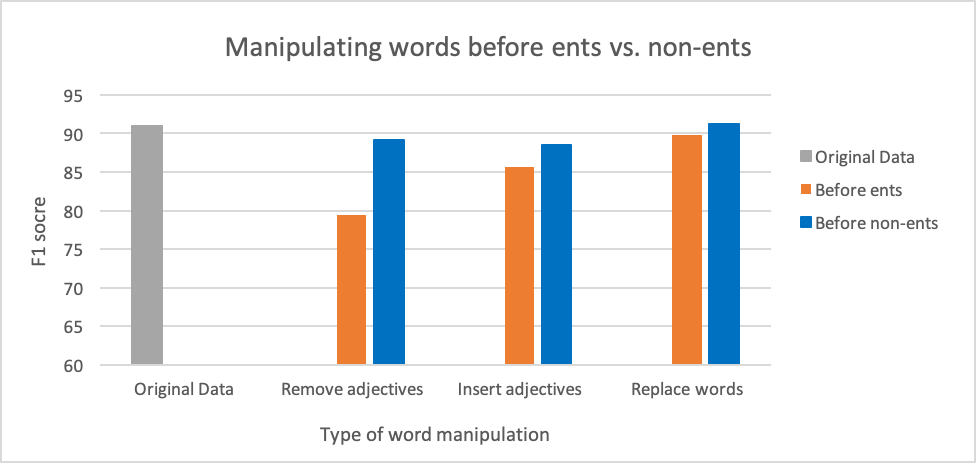
\includegraphics[width=0.85\linewidth]{LatexDiss/figures/manipentsvsnonents.png}
	\caption{Comparison of manipulating randomly-chosen words before entities versus before non-entities in context-based attacks. This experiment was performed using our baseline model and the CoNLL03 test set.}
	\label{fig:manipentsvsnonents}
\end{figure}
 
\subsubsection{Influential word selection: AllenNLP Interpret}
\label{sec:allennlpinterpret}
The first non-random way for selecting influential words that I investigate is using AllenNLP Interpret~\citep{allennlpinterpret}. AllenNLP Interpret can be applied to any differentiable NLP model. By differentiating the model and finding the gradient of the loss (with respect to the model's actual output) for each token, AllenNLP Interpret determines which input word is the most influential for the model's prediction~\citep{allennlpinterpret}. I use AllenNLP Interpret to select the top $k$ most influential words, which I manipulate through removal, insertion, and replacement.

The benefit of AllenNLP Interpret is that it takes a model-specific approach to quantitatively and definitively selecting the most influential words. However, the downside is that it requires a white-box approach to adversarial attacks, meaning that in order to develop the adversarial examples, we need to know the structure of the model at hand. Additionally, the  model has to be end-to-end differentiable so that we can calculate the gradient of the loss.

\subsubsection{Influential word selection: Cooccurrence Matrix}
% note why we compute influence on the training data only, ignoring dev and test
A cooccurrence matrix is an approach to finding influential words that is model agnostic. In this approach, I create a dictionary with every non-entity word in the corpus. For each word in the corpus, I record the number of times that it appears in the same sentence as an entity of each type. For example, the sentence ``\textit{Costco} has taken off in \textit{Canada}'' would increment the counters for each entry in the set  \{(has, \texttt{ORG}), (taken, \texttt{ORG}), (off, \texttt{ORG}), (in, \texttt{ORG}), (has, \texttt{LOC}), (taken, \texttt{LOC}), (off, \texttt{LOC}), (in, \texttt{LOC})\}. I considered ignoring stop words (words that are commonly filtered out in NLP such as ``the'', and ``and''). However, some stop words might have an association with a particular entity type. For example, ``in'' and ``at'' are highly associated with \texttt{LOC}. 

In order to determine a word's influence on the model's prediction for a sentence, I sum the word's influence over all of the sentence's entities. To determine the influence of each entity-word combination, two values must be taken into account. First we must consider how many times the word and entity type have been seen together in the same sentence throughout the corpus. This is exactly the information stored in the cooccurrence matrix. This value is important because it is likely that the model has learned which words are most often associated with a given entity type, making these words influential. For example, the word ``said'' often appears in sentences with a \texttt{PER} entity. In fact, according to the cooccurrence matrix I developed on the CoNLL03 training data, ``said'' is the word most frequently associated with \texttt{PER} besides ``the.'' 

However, neither ``said'' nor ``the'' are assigned the highest influence rating. This is because there is a second value to consider: the relative frequency of a word. If we strictly consider the frequency with which a word and entity type appear together, ``the'' would rank among the most influential words for every entity type. The relative frequency is the ratio of the frequency with which a word is associated with a specific entity type compared to the frequency of the word throughout the entire corpus. This value gives an idea of how influential a word is to a specific entity type rather than merely indicating how prevalent that word is throughout the corpus. This ratio alone is not enough to accurately represent a word's influence because extremely infrequent words would end up with a high ratio despite their lack of influence. For example, according to the cooccurrence matrix I developed on the CoNLL03 training data, the pair (``pavilion'', \texttt{PER}) has a perfect relative frequency of 1.0. However, this is because the word pavilion only appears once in the corpus. In order to accurately represent a word's influence on an entity's type, I combine these two indicators such that the influence of a specific word/entity type pair is calculated as follows:

{
    \begin{align*} 
        \operatorname{influence} = \operatorname{total\ associations} \times \operatorname{relative\ frequency}
    \end{align*} 
}

\subsubsection{Results of context-based attacks: influential word selection}
\label{sec:contextattackres}
As seen in Table~\ref{tab:influentialwords} and Fig~\ref{fig:influentialwords}, random selection of words is the most effective way to create adversarial attacks in this context-based setting and AllenNLP Interpret is the least effective. This result was surprising considering that AllenNLP Interpret leverages knowledge of the structure of the NER model. My next step is to further investigate these results, looking through the specific successful attacks to see why random selection of influential words seems most effective.

\begin{table}[h]
    \centering
    \begin{singlespace}
    \scalebox{.7} {
    \begin{tabular}{@{} R{0.5\textwidth}@{\hskip .6in} c c c | c c c @{}}
\toprule   \toprule
        & \multicolumn{3}{L{0.3\textwidth}}{\small{\textbf{Performance on dev data}}}
        & \multicolumn{3}{L{0.3\textwidth}}{\small{\textbf{Performance on test data}}} \\

        \small{\textbf{Adversarial Technique}}
        & \small{\textit{Precision}}
        & \small{\textit{Recall}}
        & \small{\textit{F1}}
        & \small{\textit{Precision}}
        & \small{\textit{Recall}}
        & \small{\textit{F1}} \\
\toprule
        \small{Original data}
            & 94.86 & 94.50 & 94.68
            & 91.03 & 90.91 & 90.97 \\
\midrule
        \small{Remove adjectives randomly before ents}
            & 89.47 & 82.93 & 86.08 
            & 80.65 & 78.12 & 79.37 \\
        \small{Remove adjectives using AllenNLP Interpret}
            & 94.39 & 93.97 & 94.18
            & 91.34 & 90.93 & 91.13 \\
        \small{Remove adjectives using cooccurrence matrix}
            & 93.54 & 93.09 & 93.31
            & 89.48 & 88.9 & 89.19 \\
\midrule
        \small{Insert adjectives randomly before ents}
            & 88.46 & 82.63 & 85.45 
            & 86.03 & 85.4 & 85.71 \\
        \small{Insert adjectives using AllenNLP Interpret}
            & 94.49 & 94.61 & 94.55
            & 90.88 & 90.79 & 90.83 \\
        \small{Insert adjectives using cooccurrence matrix}
            & 92.96 & 93.01 & 92.99
            & 88.52 & 88.55 & 88.54 \\
\midrule
        \small{Replace words randomly before ents}
            & 93.35 & 92.79 & 93.07 
            & 90.30 & 89.33 & 89.81 \\
        \small{Replace words using AllenNLP Interpret}
            & 95.35 & 95.18 & 95.26
            & 92.89 & 92.12 & 92.50 \\
        \small{Replace words using cooccurrence matrix}
            & 94.97 & 94.55 & 94.76
            & 92.14 & 91.76 & 91.95 \\
\hline
    \end{tabular}
    }
    \end{singlespace}
    \caption{Comparison of techniques for choosing influential words for context-based attacks. This experiment was performed using our baseline model and the CoNLL03 dataset.}
    \label{tab:influentialwords}
\end{table}
 
 \begin{figure}[h]
	\centering
	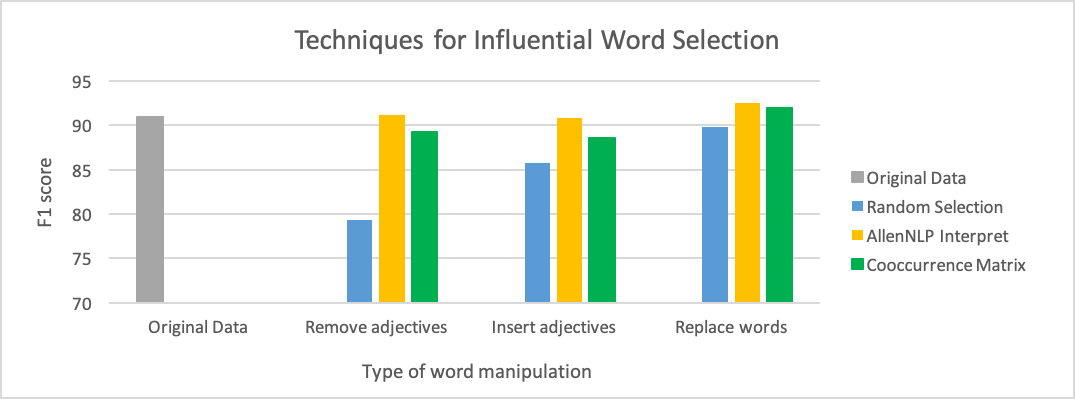
\includegraphics[width=0.85\linewidth]{LatexDiss/figures/influentialwords.png}
	\caption{Comparison of techniques for choosing influential words for context-based attacks. This experiment was performed using our baseline model and the CoNLL03 test set.}
	\label{fig:influentialwords}
\end{figure}

\section{Adversarial Training Experiments}
Although the main purpose of the adversarial augmentation techniques was to \textit{test} the robustness of a model, they can also be used to \textit{improve} the robustness of the model to these same types of adversarial attacks. In this section, I investigate the efficacy of adversarial training using the adversarial augmentation techniques described in Sec~\ref{sec:advattackexp}. 

\subsection{Adversarial Training Technique}
Adversarial training uses the same augmentation scripts as were used for adversarial attacks. The first step is to use these scripts on the training and dev data. For each adversarial augmentation technique, I make an augmented training file that includes the original training data as well as the augmented training data. I make an augmented dev file in the same manner. I then train a new NER model (of the same BLSTM-CRF structure as the baseline model) on this augmented training data. Finally, I test the augmented model's performance on the adversarial test dataset in order to evaluate whether the adversarial training improved the model's robustness to the adversarial attack. Additionally, I test the augmented model's performance on the original CoNLL03 test dataset to evaluate whether the adversarial training was detrimental to the model's success on the original data.

\subsection{Adversarial Training Results}
As seen in Table~\ref{tab:advtraining} and Fig~\ref{fig:advtraining}, the augmented NER models' performance on the adversarial test dataset tends to be higher than the original baseline model, demonstrating the efficacy of adversarial training. Further, as seen in Table~\ref{tab:advtraining} and Fig~\ref{fig:augmodelsorigdata}, this improvement comes without a significant decrease in performance on the original test dataset, evidencing that adversarial training increases the model's robustness without harming its performance on standard data. For brevity, I only present the adversarial training results on the most successful entity-based and context-based attacks. However, the other augmentation techniques produce a similar pattern.

\newpage

\begin{table}[h]
    \centering
    \begin{singlespace}
    \scalebox{.7} {
    \begin{tabular}{@{} R{0.35\textwidth}@{\hskip .6in} c c c | c c c | c c c @{}}
\toprule   \toprule
        & \multicolumn{3}{C{0.3\textwidth}}{\small{\textbf{Original model on adversarial data}}}
        & \multicolumn{3}{C{0.3\textwidth}}{\small{\textbf{Augmented model on adversarial data}}} 
        & \multicolumn{3}{C{0.3\textwidth}}{\small{\textbf{Augmented model on original data}}} \\

        \small{\textbf{Augmentation Type}}
        & \small{\textit{Precision}}
        & \small{\textit{Recall}}
        & \small{\textit{F1}}
        & \small{\textit{Precision}}
        & \small{\textit{Recall}}
        & \small{\textit{F1}} 
        & \small{\textit{Precision}}
        & \small{\textit{Recall}}
        & \small{\textit{F1}} \\
\toprule
        \small{Original model on original data}
            & - & - & -
            & - & - & -
            & 91.03 & 90.91 & 90.97 \\
\midrule
        \small{All ents fully masked}
            & 63.94 & 59.54 & 61.66 
            & 76.02 & 76.49 & 76.25 
            & 89.63 & 90.16 & 89.89 \\
        \small{All ents half masked}
            & 66.16 & 62.20 & 64.12 
            & 77.56 & 77.71 & 77.63 
            & 90.38 & 90.78 & 90.58 \\
        \small{All ents masked, retain vowels}
            & 64.68 & 60.82 & 62.69 
            & 75.55 & 76.03 & 75.79 
            & 90.37 & 91.02 & 90.69 \\
        \small{One ent fully masked}
            & 85.68 & 83.60 & 84.63 
            & 88.13 & 88.19 & 88.16 
            & 90.47 & 91.25 & 90.86 \\
        \small{One ent half masked} 
            & 86.12 & 84.23 & 85.16
            & 88.60 & 88.73 & 88.66 
            & 90.66 & 91.64 & 91.15 \\
        \small{One ent masked, retain vowels}
            & 85.62 & 83.77 & 84.68
            & 88.22 & 88.06 & 88.14 
            & 90.52 & 91.27 & 90.89 \\
\midrule
        \small{Remove adjectives}
            & 80.65 & 78.12 & 79.37 
            & 77.42 & 75.00 & 76.19 
            & 91.36 & 90.93 & 91.14 \\
        \small{Insert adjectives}
            & 86.03 & 85.40 & 85.71 
            & 88.41 & 89.05 & 88.73 
            & 91.24 & 90.88 & 91.06 \\
        \small{Replace words}
            & 90.30 & 89.33 & 89.81
            & 90.79 & 90.61 & 90.70 
            & 90.75 & 91.18 & 90.97 \\
\hline
    \end{tabular}
    }
    \end{singlespace}
    \caption{Comparison of the original model's performance and augmented model's performance on adversarial datasets based on the CoNLL03 dataset. Related words were chosen using BERT. Influential words are selected as random words before entities.}
    \label{tab:advtraining}
\end{table}

\vspace{75px}
 
 \begin{figure}[h]
	\centering
	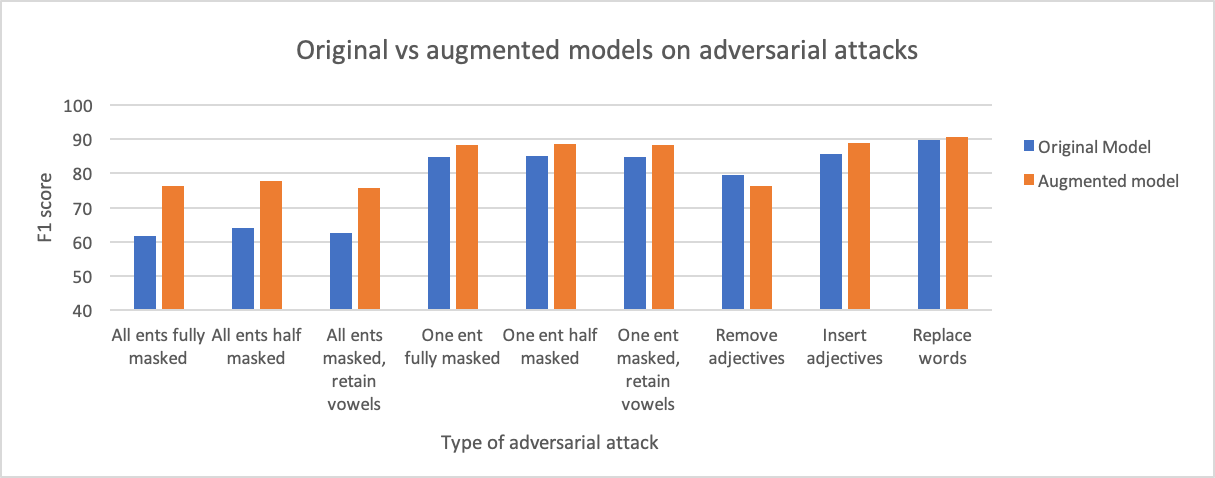
\includegraphics[width=0.85\linewidth]{LatexDiss/figures/advtraining.png}
	\caption{Comparison of the original model's performance and augmented model's performance on adversarial datasets based on the CoNLL03 dataset. Related words were chosen using BERT. Influential words are selected as random words before entities.}
	\label{fig:advtraining}
\end{figure}

 \begin{figure}[h]
	\centering
	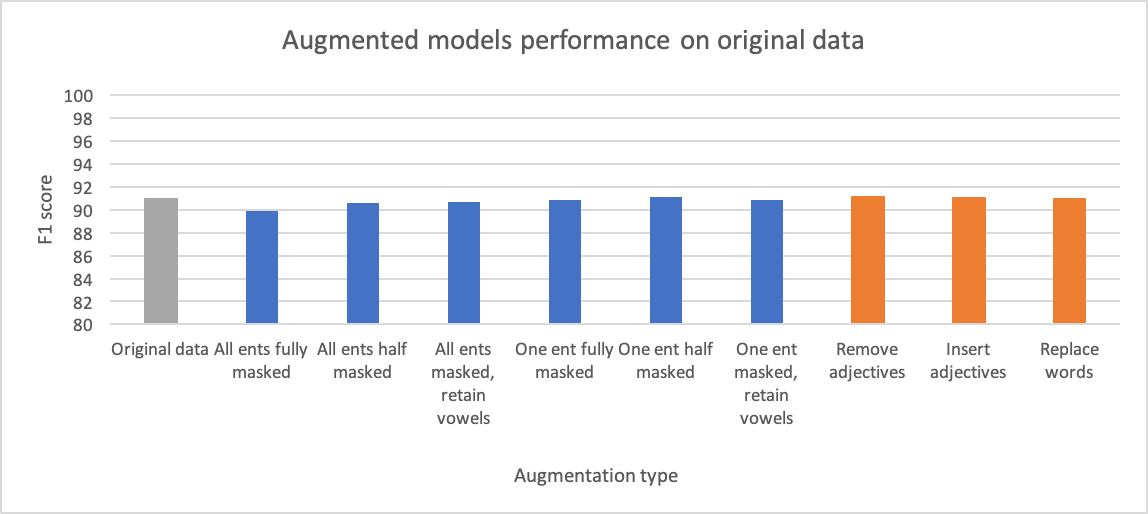
\includegraphics[width=0.85\linewidth]{LatexDiss/figures/augmodelsorigdata.png}
	\caption{Comparison of the augmented models' performance and the original model's performance on the original CoNLL03 test dataset. Related words were chosen using BERT. Influential words are selected as random words before entities.}
	\label{fig:augmodelsorigdata}
\end{figure}

\newpage

\section{Future Directions}
This is an ongoing project. One of my next steps is to thoroughly examine the results from context-based attacks presented in Sec~\ref{sec:contextattackres} to investigate why random selection of influential words was more effective than systematic selection. I also plan to continue developing the related word selection with BERT by using suggested words with a lower confidence score in the hopes that they are more likely to fool the baseline model because they are less common words.

More generally, I plan to apply these adversarial augmentation techniques to other NER datasets. CoNLL03 is a limited dataset because it is relatively simplistic, containing only four categories of named entities. Further, the CoNLL03 dataset contains many labeling mistakes. In particular, because the dataset contains many sporting event results, there are many discrepancies as to whether a country name such as ``Japan'' should be counted as an \textsc{LOC} or \textsc{ORG} in the context of a sports team.

I would also like to run human experiments to ensure that the adversarial data is able to be labeled by humans. Evidence that humans can properly label the adversarial data would confirm that the adversarial data is in fact valid.

% could we incorporate IBP?
% genetic algorithms as in Alzentot rather than random perturb (they got from 52\%  to 97\%)

